\section{Типы галактик, эволюция галактик}

\subsection{Типы галактик}

Галактики согласно классификации Хаббла делятся на эллиптические (E), спиральные (S) и неправильные (Irr). Примеры красивых картинок можно найти на рисунке \ref{fig:16_galaxy_types}.

\begin{figure}[H]
	\centering
	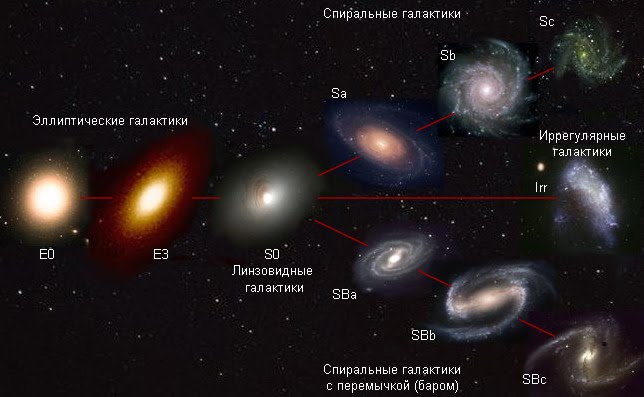
\includegraphics[width=0.9\linewidth]{16_galaxy_types}
	\caption{Типы галактик: эллиптические (E), спиральные (S) и неправильные (Irr)}
	\label{fig:16_galaxy_types}
\end{figure}

\subsubsection{Эллиптические галактики}

Эллиптические галактики имеют эллиптическую форму и характеризуются равномерной яркостью, которая постепенно убывает от края к центру.

Форма галактик данного типа варьируется от практически совершенно круглой, до сплюснутого эллипса. Соответственно для обозначения степени сплюснутости галактики к букве Е прибавляется число n, определяемое по формуле: $n = 10 (a - b) / a$, где $ a$, $b$, - это соответственно большая и малая полуоси галактики. Таким образом, эллиптическая галактика круглой формы будет отнесена к типу Е0, а сплюснутая может быть классифицирована, например, как $E3$.

\subsubsection{Спиральные галактики}

В спиральных галактиках ядро представляет собой наиболее яркую область, обладающую признаками эллиптических галактик. Наличие в спиральной галактике перемычки (бара) позволяет разделить их на два основных типа. К первому относятся нормальные спиральные галактики, обозначаемые буквой (S). Ко второму типу относятся так называемые пересеченные галактики, обозначаемые (SB). Для более точной характеристики той или иной галактики, деления их всего на 2 типа недостаточно. Поэтому Хаббл классифицировал спиральные галактики по следующим трем критериям:

\begin{enumerate}
	\item Относительной величине ядра, по сравнению с размерами всей галактики;
	
	\item По тому, насколько сильно или слабо закручены спиральные ветви;
	
	\item Фрагментарности спиральных ветвей.
\end{enumerate}

К типу Sa или (SBa) относятся галактики с очень обширной ядерной областью и сильно закрученными спиральными ветвями - непрерывными и гладкими, а не фрагментарными.

Галактики типа Sb и SBb имеют относительно небольшую ядерную область, и не очень сильно закрученные спиральные ветви, которые разрешаются на отдельные яркие фрагменты. Галактики типа Sc и SBc характеризуются сильно фрагментарными обрывочными спиральными рукавами. У галактик SBc даже бар разделяется на отдельные фрагменты.

Кроме того, отдельно выделен тип галактик, промежуточный, между спиралями и эллиптическими системами, - галактики типа SO. У них чрезвычайно толстый диск, мощный балдж и не видно спиральных ветвей. Кстати, обозначив этот тип галактик буквой S, несмотря на отсутствие спиралей, Хаббл тем самым подчеркнул, что главным в различии спиральных и эллиптических систем является звездный диск.

\subsection{Эволюция галактик}
Единой теории образования и эволюции галактик нет. Возможные теории образования галактик:
\begin{itemize}
	\item \textbf{Иерархическая теория} предполагает, что уже после возникновения первых звёзд во Вселенной начался процесс гравитационного объединения звёзд в скопления и далее в галактики. 
	
	Недостаток: современные наблюдения показывают, что на \(z \approx 10\) (спустя 400 млн после Большого взрыва) уже существовали сформировавшиеся галактики, но между возникновением первых звезд и вышеуказанным периодом прошло слишком мало времени, так что галактики сформироваться не успели бы.
	
	\item \textbf{Инфляционная теория}. Во время расширения вселенной со сверхсветовой скоростью (инфляционного расширения) происходили квантовые флуктуации. Квантовые флуктуации расширялись вместе со всей вселенной, причем до порядков, в \(10^{10^{12}}\) раз превышающих исходный. Те из них, которые существовали в момент прекращения инфляции, остались <<раздутыми>> и оказались первыми тяготеющими неоднородностями во Вселенной. Получается, что у материи было порядка 400 млн лет на гравитационное сжатие вокруг этих неоднородностей и образование газовых туманностей. А далее начался процесс возникновения звёзд и превращения туманностей в галактики.
\end{itemize}

В процессе эволюции галактики могут сливаться друг с другом. Результатом слияния галактик, как правило, оказываются эллиптические галактики. В пользу этого говорит тот факт, что звезды в эллиптических галактиках находятся на орбитах, случайно ориентированных внутри галактик.

Прекращение процесса звездообразования в галактиках называется <<тушением галактик>>. Звезды образуются из холодного газа, поэтому галактика гаснет, когда в ней больше нет холодного газа. Однако считается, что тушение происходит относительно быстро (в течение 1 миллиарда лет), что намного меньше времени, которое потребуется галактике, чтобы просто израсходовать свой резервуар холодного газа. Модели эволюции галактик объясняют это гипотезой о других физических механизмах, которые устраняют или перекрывают подачу холодного газа в галактику. Эти механизмы можно в общих чертах разделить на две категории:

\begin{itemize}
	\item Механизмы \textbf{превентивной} обратной связи, которые не позволяют холодному газу проникать в галактику или не дают ему образовывать звезды. Стройной физической концепции нет.
	
	\item Механизмы \textbf{выталкивающей} обратной связи, которые удаляют газ так, чтобы он не мог образовывать звезды. Один из механизмов выброса  вызван сверхмассивными черными дырами, обнаруженными в центрах галактик. Моделирование показало, что газ, аккрецирующий на сверхмассивных черных дырах в центрах галактик, производит струи высокой энергии; высвобожденная энергия может вытеснить достаточно холодного газа, чтобы погасить звездообразование.
\end{itemize}